% ! TeX root = ../bachelor-thesis.tex

\chapter{Studio del problema}
\label{ch:Chapter2}

In questo capitolo si analizzerà la natura del problema che si vuole risolvere,
identificando i requisiti che il sistema dovrà soddisfare per adempiere al suo
scopo.

Nello specifico, si formalizzeranno le funzioni che il sistema deve poter
assolvere, classificandole in base alla loro priorità. Inoltre, si discuteranno
quei vincoli del sistema che dipendono dalla sua stessa natura.

\section{Analisi dei requisiti}
\label{sec:Sezione2.1}

Ora si descriveranno in un modo più ordinato e formale i requisiti del sistema
da progettare.

Più in dettaglio, i requisiti saranno categorizzati attraverso la
prioritizzazione MoSCoW \cite{MOSCOW}. Si distingueranno quindi i requisiti
\textit{must have}, ovvero quelli vitali, che devono essere soddisfatti dal
sistema a breve termine, i requisiti \textit{should have}, ovvero quelli
importanti, che dovranno essere soddisfatti dal sistema a lungo termine, e i
requisiti \textit{could have}, ovvero quelli opzionali, che potranno essere
integrati una volta ultimato il sistema. In questa tesi progettuale, lo scopo
preposto è quello di soddisfare almeno i requisiti \textit{must have}, quindi
tutti gli schemi trattati, faranno riferimento esclusivamente a quei requisiti.

\subsection{Must Have}
\label{subsec:Sezione2.1.1}

Il sistema dovrà assolutamente soddisfare i seguenti requisiti funzionali:

\begin{enumerate}
  \item[\textbf{A.}] \textit{\textbf{Controllo dei dispositivi domotici da
            sistema di controllo.}} Sarà necessario fornire all’utente un
        sistema di controllo, attraverso il quale si potrà interagire per
        monitorare e controllare i propri dispositivi domotici.
  \item[\textbf{B.}] \textit{\textbf{Controllo dei dispositivi domotici
            attraverso comandi vocali.}} Sarà necessario fornire all’utente
        un’assistente vocale, integrato con il sistema di controllo domotico,
        attraverso il quale si potrà controllare i propri dispositivi domotici
        attraverso comandi vocali.
  \item[\textbf{C.}] \textit{\textbf{Ricezione delle notifiche dai dispositivi
            domotici.}} Sarà necessario fornire all’utente la possibilità di
        ricevere delle notifiche sugli eventi rilevati dai dispositivi
        domotici, sia tramite il sistema di controllo domotico, sia tramite
        l’assistente vocale (quando più opportuno).
  \item[\textbf{D.}] \textit{\textbf{Accesso allo storico degli eventi rilevati
            dai dispositivi domotici.}} Sarà necessario registrare tutti gli
        eventi rilevati dai dispositivi domotici fino a un certo periodo di
        tempo, così da fornire all’utente la possibilità di consultare lo
        storico degli eventi tramite il sistema di controllo domotico.
  \item[\textbf{E.}] \textit{\textbf{Accesso ad almeno tre giochi cognitivi
            distinti tramite l’assistente vocale.}} Sarà necessario fornire
        all’utente un servizio comprendente almeno tre giochi cognitivi tra
        cui poter scegliere e a cui poter accedere attraverso l’assistente
        vocale. I giochi cognitivi dovranno distinguersi in base alle
        capacità cognitive di cui permetteranno l’allenamento.
\end{enumerate}

Di seguito, il diagramma dei casi d’uso che schematizza questi specifici
requisiti, che saranno quelli trattati successivamente nella tesi (Figura
\ref{fig:figure2.1}).

\begin{figure}[H]
  \centering
  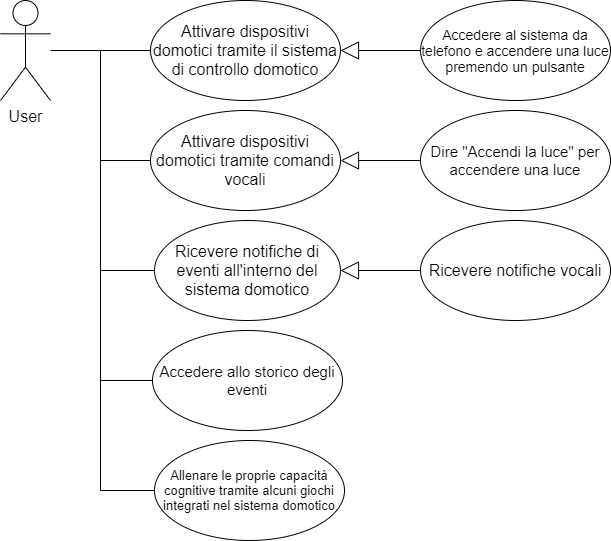
\includegraphics[scale=0.5]{resources/images/analysis/use-cases-diagram.jpg}
  \caption{
    Il diagramma dei casi d'uso che riassume i requisiti funzionali del
    sistema.
  }
  \label{fig:figure2.1}
\end{figure}

\subsection{Should Have}
\label{subsec:Sezione2.1.2}

In un secondo momento, il sistema dovrà evolversi soddisfacendo i seguenti
requisiti funzionali:

\begin{enumerate}
  \item[\textbf{F.}] \textit{\textbf{Gestione dell’autenticazione come paziente
            o personale socio-sanitario.}} Sarà necessario gestire
        l’autenticazione, introducendo delle credenziali per essere
        riconosciuti come pazienti o come personale socio-sanitario.
  \item[\textbf{G.}] \textit{\textbf{Accesso allo storico dei risultati
            ottenuti sui diversi giochi cognitivi di un determinato paziente.}}
        Sarà necessario registrare il risultato ottenuto dal paziente alla fine
        di ciascuna partita, per ogni gioco cognitivo, così da fornire un
        campione di dati analizzabile per monitorare e comprendere i
        miglioramenti conseguiti dal paziente. Questo storico sarà accessibile
        solo a personale socio-sanitario autorizzato.
  \item[\textbf{H.}] \textit{\textbf{Analisi dei risultati ottenuti sui diversi
            giochi cognitivi.}} Sarà necessario implementare un servizio,
        possibilmente scalabile, che potrà accedere ai risultati ottenuti
        da uno specifico paziente, così da poter eseguire un’analisi più
        dettagliata dei risultati del paziente e produrre un report dei
        progressi, visualizzabile dal personale socio-sanitario
        autorizzato.
  \item[\textbf{I.}] \textit{\textbf{Gestione del percorso educativo di un
            paziente.}} Sarà necessario permettere al personale socio-sanitario
        autorizzato d'impostare un percorso educativo per un dato
        paziente, che preveda una routine di giochi cognitivi, da proporre
        a tale paziente attraverso l’assistente vocale.
  \item[\textbf{J.}] \textit{\textbf{Aggiunta di nuovi giochi cognitivi.}}
        Sarà necessario espandere il servizio che fornisce i giochi cognitivi,
        in modo da coprire più capacità cognitive, ma anche fornire più varietà
        per allenare la stessa capacità cognitiva.
\end{enumerate}

\subsection{Could Have}
\label{subsec:Sezione2.1.3}

Di seguito, i requisiti considerati opzionali, ovvero che potrebbero essere
implementati nei tempi successivi al completamento del sistema:

\begin{enumerate}
  \item[\textbf{K.}] \textit{\textbf{Accesso ai giochi cognitivi al di fuori
            del contesto socio-sanitario.}} Sarà opzionale consentire l’accesso
        ai giochi cognitivi al di fuori del contesto socio-sanita\-rio, così
        da poterli installare su altri sistemi domotici pubblici o privati.
  \item[\textbf{L.}] \textit{\textbf{Suggerimento casuale di un gioco
            cognitivo.}} Sarà opzionale permettere all’assistente vocale di
        proporre all’utente uno dei giochi cognitivi installati, a discrezione
        dell’utente.
  \item[\textbf{M.}] \textit{\textbf{Ulteriore aggiunta di nuovi giochi
            cognitivi.}} Sarà opzionale espandere nuovamente il servizio che
        fornisce i giochi cognitivi, in modo da coprire più capacità cognitive,
        ma anche fornire più varietà per allenare la stessa capacità cognitiva.
\end{enumerate}

\section{Vincoli del Sistema}
\label{sec:Sezione2.2}

Ora si illustreranno alcuni dei vincoli del sistema, dovuti alla natura del
sistema stesso.

Il primo vincolo è dovuto ai \textbf{costi}. Infatti configurare un sistema
domotico, che sia un impianto o una \textit{smart home} (o entrambi), ha dei
costi non irrisori per l’acquisto dei dispositivi, soprattutto se si tratta di
dispositivi progettati per l’accessibilità.

Il secondo vincolo è dovuto all’uso di un assistente vocale. Gli assistenti
vocali si basano su \textit{cloud computing}, che ha enormi vantaggi in termini
di fruibilità di risorse e scalabilità, tuttavia ha anche qualche svantaggio.

In primo luogo, gli assistenti vocali necessitano di una connessione a
Internet, anzi più specificamente necessitano di una \textbf{connessione verso
il cloud del produttore}. In altre parole, se, per un qualche motivo, un giorno
non è possibile raggiungere il cloud del produttore, quel giorno l’assistente
vocale non potrà funzionare (perciò non si potrà accedere ai giochi cognitivi,
né utilizzarlo per controllare il proprio sistema domotico).

In secondo luogo, vi è la questione della \textbf{privacy} e della
\textbf{sicurezza}. Infatti, gli assistenti vocali inviano le registrazioni
vocali al cloud del produttore per essere processate e dunque interpretate come
linguaggio parlato. Questo chiaramente richiede un alto livello di fiducia da
parte dell’utilizzatore. Risulta quindi necessaria un’infrastruttura di rete
sicura e un rispetto adeguato delle norme di privacy e sicurezza da parte dei
produttori.

Fortunatamente, molti produttori hanno recentemente adottato un’infrastruttura
che promuova l’\textit{edge computing}, ovvero una forma di cloud computing,
che sposta i centri di calcolo verso gli utilizzatori, riducendo il tempo per
cui i loro dati si trovano in rete e migliorando anche la responsività e
fruibilità dei servizi forniti, tra cui gli assistenti vocali.

Un terzo e ultimo vincolo è infine dovuto alla natura dei giochi, che si basano
strettamente su interazioni vocali. Ciò rende \textbf{difficile realizzare
giochi troppo complessi}, in cui la quantità d'informazioni da scambiare è
molto elevata. In questi giochi, infatti, risulterebbe più efficace una
comunicazione parallela, basata su più sensi (come vista e udito), piuttosto
che una seriale, come un’interazione vocale, che si basa solo sull’udito. Per
fortuna però, molti esercizi cognitivi si basano su interazioni semplici e si
prestano piuttosto bene a essere implementati attraverso un’assistente vocale.
